\section{Related Work}
\label{sec:related_work}

% First Daugman's ideas 
The first ideas for countermeasures against iris presentation attacks were proposed some 18 years ago by Daugman \cite{Daugman_IMAIP_2000} and became a basis of many current effective PAD methods. Early Daugman's concepts include finding anomalies in Fourier spectrum to detect printed irises, either on a paper or on a contact lens, detection of specular ``Purkinje'' reflections from both the cornea and the lens, or investigating pupil size variations, either spontaneous (``hippus'') or stimulated by visible light.

% Vulnerabilities
In general, there are two goals in presentation attacks, impersonation or identity concealment. The first successful demonstration of impersonation with the use of a commercial sensor was shown by Thalheim \etal \cite{Thalheim_CT_2002}. They used iris images printed on a paper, with a hole cut where the pupil was printed, to make a successful impersonation attack on a commercial iris recognition system with authentic eyes previously enrolled. The first use of one's eye to evade recognition observed in an operational environment was recorded at the border crossing point employing iris recognition in the United Arab Emirates \cite{Al-Raisi_TI_2008}. The attackers administered eye drops to make the pupil excessively dilated. This made the iris texture deformed too severely to be compensated by feature extraction and matching algorithms, and hence generating false non-matches. Since these early demonstrations of vulnerabilities, other presentation attack instruments have been studied, including use of textured contact lenses that partially occlude the actual iris texture \cite{Doyle_ICB_2013}, presentation of iris images displayed on a screen \cite{HeXiaofu_ICB_2009}, or use of prosthetic eyes \cite{Zuo_TIFS_2007}. After recent studies by Trokielewicz \etal \cite{Trokielewicz_BTAS_2016} presenting that post-mortem iris recognition is possible for a couple of weeks after death, cadaver eyes can also be considered as a potential presentation attack instrument.

% THIS FIGURE IS FOR THE NEXT SECTION (PROPOSED METHOD)
%
\begin{figure*}[!tb]
    \begin{subfigure}[b]{0.32\linewidth}
            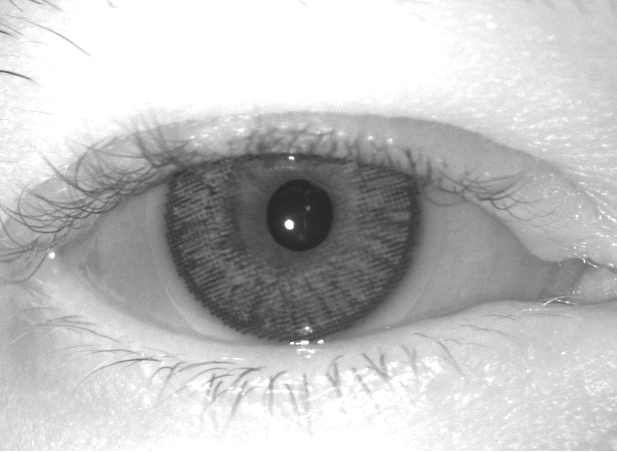
\includegraphics[width=\linewidth]{04261d2312}
        \caption{Raw iris image}
        \label{fig:origimg}
    \end{subfigure}
    ~
    \begin{subfigure}[b]{0.32\linewidth}
        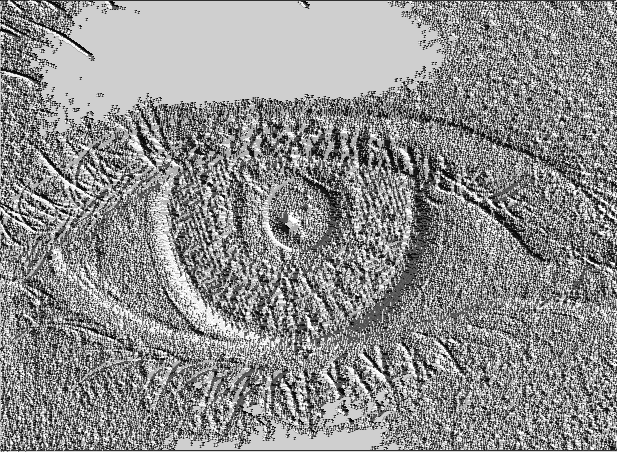
\includegraphics[width=\linewidth]{3x3x5}
        \caption{$B_{3\times 3 \times 5}$}
        \label{fig:bsif3x3}
    \end{subfigure}
    ~
    \begin{subfigure}[b]{0.32\linewidth}
        \centering
        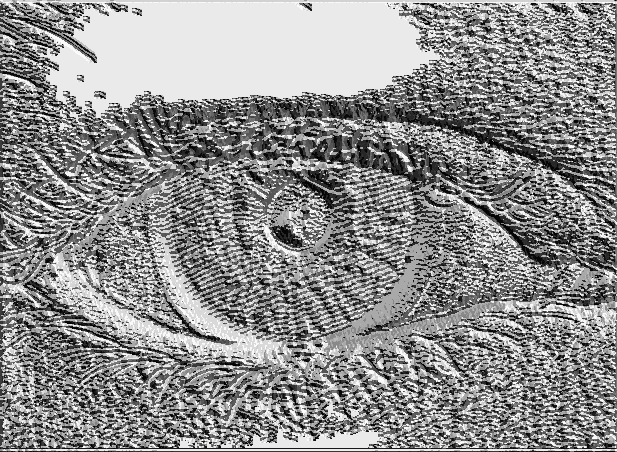
\includegraphics[width=\linewidth]{7x7x12}
        \caption{$B_{7\times 7 \times 12}$}
        \label{fig:bsif7x7}
    \end{subfigure}
    \caption{Examples of different BSIF representations $B_{n\times n \times l}$ (\ref{fig:bsif3x3},\ref{fig:bsif7x7}) of the same image (\ref{fig:origimg}). Note how the structure of the contact lens is highlighted through the different representations.}
    \label{fig:bsif_examples}
\end{figure*}


% Literature overview depending on the sophistication of the PAD method
There is a rich literature on PAD methods presenting various levels of sophistication, and putting different requirements on the sensors' configuration and signals necessary to detect presentation attacks. In the largest group of PAD methods, a single near-infrared iris image, compliant to ISO/IEC 19794-6, is used in both identity verification and presentation attack detection. The \emph{hand-crafted} approaches use various image descriptors to calculate image features, which are used to distinguish between authentic irises and artifacts typically through the use of Support Vector Machine classifiers. Popular techniques used in calculation of PAD-related iris image features are Binarized Statistical Image Features (BSIF) \cite{Komulainen_IJCB_2014}, Local Binary Patterns (LBP) \cite{Doyle_ICB_2013}, Binary Gabor Patterns (BGP) \cite{Lovish_CAIP_2015}, Local Contrast-Phase Descriptor (LCPD) \cite{Gragnaniello_TIFS_2015}, Local Phase Quantization (LPQ) \cite{Sequeira_TSP_2016}, Scale Invariant Descriptor (SID) \cite{Gragnaniello_SITIS_2014}, Scale Invariant Feature Transform (SIFT) and DAISY \cite{Pala_CVPR_2017}, Locally Uniform Comparison Image Descriptor (LUCID) and CENsus TRansform hISTogram (CENTRIST) \cite{Akhtar_AVSS_2014}, Weber Local Descriptor (WLD) \cite{Gragnaniello_TIFS_2015}, Wavelet Packet Transform (WPT) \cite{Chen_PRL_2012} or image quality descriptors proposed by Galbally \etal \cite{Galbally_Handbook_2016}. Instead of ``hand-crafting'' effective feature extractors, one may also benefit from recently popular \emph{data-driven} approaches that learn directly from the data how to process and classify iris images to solve the PAD task  \cite{Silva_SIBGRAPI_2015,Menotti:TIFS:2015,Gragnaniello_SITIS_2016,He_BTAS_2016,Pala_CVPR_2017,Raghavendra_WACV_2017}. 

The above PAD methods rely upon an iris image that is typically used later for biometric recognition, and hence they can be implemented in the existing iris recognition sensors. However, if some hardware adaptations are possible, and some more complicated static features of the eye can be measured, one may consider multi-spectral analysis \cite{Lee_BS_2006,Park_OptEng_2007,Chen_PRL_2012,Thavalengal_TCE_2016} or estimation of three-dimensional iris features \cite{Pacut_ICCST_2006,Lee_IMA_2010,Connell_ASSP_2013,Hughes_HICSS_2013} as potential PAD techniques. Making the PAD more complex, one may consider measuring spontaneous dynamic features of the eye, such as micro-movements of an eyeball, either using Eulerian video magnification \cite{Raja_TIFS_2015} or by using an eye-tracking device \cite{Rigas_PRL_2015}. If there is a possibility to additionally stimulate the eye with varying visible light, and measure its reaction, the use of pupil dynamic models may help to easily detect static or oddly-behaving artifacts \cite{Czajka_TIFS_2015,Thavalengal_TCE_2016}. A recent survey  by Czajka and Bowyer provides a comprehensive assessment of the state of the art in iris PAD \cite{Czajka_CSUR_2018}.

In \cite{Nguyen_2018}, a PAD approach based on deep features extracted from different iris regions and classified by feature and score-level fusion of SVM is described. The authors report very low error rates on a subset of the LivDet-Iris 2017 datasets.
Kontschieder \etal \cite{kontschieder2015deep} published a work that seeks to combine deep convolutional networks for feature extraction, with the classification power of Random Forests. They describe an alternative approach to train Random Forest classifiers, which consists of a stochastic version of decision trees that are trainable through backpropagation. Random Forests trained with this method can either be standalone classifiers or act as alternative classifiers on top of a CNN. The authors claim to have outperformed the state of the art in image classification when integrating it to a GoogLeNet network.

% Standards, and LivDet as a the most recent benchmark
Evaluation of PAD reliability significantly differs from statistical evaluation of biometric recognition. ISO/IEC JTC1 subcommittee 37 issued both the PAD-related vocabulary \cite{ISO_30107-1_2016}, and recommendations on how to evaluate and report the PAD-related performance \cite{ISO_30107-3_2017}. An important effort related to iris PAD evaluation is the LivDet-Iris competition series (\url{http://livdet.org/}), which has had editions in 2013 \cite{Yambay2014}, 2015 \cite{Yambay2015} and 2017 \cite{Yambay2017}. The  2017 edition of LivDet-Iris is the most recent, global, independent evaluation of PAD algorithms for detection of iris printouts and textured contact lenses. This paper follows exactly the LivDet-Iris 2017 evaluation protocol, and the results presented herein are directly comparable with the LivDet-Iris 2017 winning solution.